% answers.tex —— 2006 年·普通高等学校招生考试·浙江卷文科 · 参考答案与详细解析片段
% 由 tools/generate_projects.py 依来源总账自 2006/2006_数学真题_浙江文_试题.md + 2006/2006_数学真题_浙江文_解析正文.md + 2006/2006_数学真题_浙江文_答案要点.md 生成，勿手改（改源 MD 后重跑）


\begin{gktip}
以下逐题推导依据固定 PDF 题面独立完成并复算；不是官方解析。来源身份未认证。
\end{gktip}

\begin{answer}
\gksolhead{1}{}

\textbf{题目}：

设集合 $A=\{x\mid -1\leqslant x\leqslant 2\}$，$B=\{x\mid 0\leqslant x\leqslant 4\}$，则 $A\cap B=$\mbox{（　　）}

（A）$[0,2]$　（B）$[1,2]$　（C）$[0,4]$　（D）$[1,4]$

\Needspace{4\baselineskip}
\textbf{解析}

$A=[-1,2]$，$B=[0,4]$，交集为 $[0,2]$，选 A。

\gkanswer{答案：A。}

\end{answer}
\begin{answer}
\gksolhead{2}{}

\textbf{题目}：

在二项式 $(x+1)^6$ 的展开式中，含 $x^3$ 的项的系数是\mbox{（　　）}

（A）$15$　（B）$20$　（C）$30$　（D）$40$

\Needspace{4\baselineskip}
\textbf{解析}

$(x+1)^6$ 中 $x^3$ 项系数为 $\binom63=20$，选 B。由二项式定理各项系数和为 $2^6=64$，该项系数与展开式相符。

\gkanswer{答案：B，$20$。}

\end{answer}
\begin{answer}
\gksolhead{3}{}

\textbf{题目}：

抛物线 $y^2=8x$ 的准线方程是\mbox{（　　）}

（A）$x=-2$　（B）$x=-4$　（C）$y=-2$　（D）$y=-4$

\Needspace{4\baselineskip}
\textbf{解析}

标准式 $y^2=4px$ 中 $4p=8$，故 $p=2$，准线为 $x=-p=-2$，选 A。

\gkanswer{答案：A。}

\end{answer}
\begin{answer}
\gksolhead{4}{}

\textbf{题目}：

已知 $\log_{\frac12}m<\log_{\frac12}n<0$，则\mbox{（　　）}

（A）$n<m<1$　（B）$m<n<1$　（C）$1<m<n$　（D）$1<n<m$

\Needspace{4\baselineskip}
\textbf{解析}

底数 $1/2$ 在 $(0,+\infty)$ 上的对数函数递减。由 $\log_{1/2}m<\log_{1/2}n$ 得 $m>n$；两对数均小于 $0$，故 $m,n>1$。因此 $1<n<m$，选 D。

\gkanswer{答案：D。}

\end{answer}
\begin{answer}
\gksolhead{5}{}

\textbf{题目}：

设向量 $\boldsymbol a,\boldsymbol b,\boldsymbol c$ 满足 $\boldsymbol a+\boldsymbol b+\boldsymbol c=\boldsymbol 0$，$\boldsymbol a\perp\boldsymbol b$，$|\boldsymbol a|=1$，$|\boldsymbol b|=2$，则 $|\boldsymbol c|^2=$\mbox{（　　）}

（A）$1$　（B）$2$　（C）$4$　（D）$5$

\Needspace{4\baselineskip}
\textbf{解析}

由 $\boldsymbol c=-(\boldsymbol a+\boldsymbol b)$ 及正交条件，$|\boldsymbol c|^2=|\boldsymbol a|^2+|\boldsymbol b|^2=1+4=5$，选 D。

\gkanswer{答案：D，$5$。}

\end{answer}
\begin{answer}
\gksolhead{6}{}

\textbf{题目}：

函数 $f(x)=x^3-3x^2+2$ 在区间 $[-1,1]$ 上的最大值是\mbox{（　　）}

（A）$-2$　（B）$0$　（C）$2$　（D）$4$

\Needspace{4\baselineskip}
\textbf{解析}

$f'(x)=3x(x-2)$。在 $[-1,0]$ 上 $f'(x)\ge0$，在 $[0,1]$ 上 $f'(x)\le0$，故最大值在 $x=0$ 处取得。$f(0)=2$，而 $f(-1)=-2,f(1)=0$，所以最大值为 $2$，选 C。端点复算均不超过临界点值。

\gkanswer{答案：C，$2$。}

\end{answer}
\begin{answer}
\gksolhead{7}{}

\textbf{题目}：

“$a>0,b>0$”是“$ab>0$”的\mbox{（　　）}

（A）充分而不必要条件　（B）必要而不充分条件

（C）充分必要条件　（D）既不充分也不必要条件

\Needspace{4\baselineskip}
\textbf{解析}

$a>0,b>0$ 必有 $ab>0$，所以是充分条件；但 $ab>0$ 还允许 $a,b$ 同为负数，故不必要，选 A。

\gkanswer{答案：A。}

\end{answer}
\begin{answer}
\gksolhead{8}{}

\textbf{题目}：

如图，正三棱柱 $ABC-A_1B_1C_1$ 的各棱长都 $2$，$E,F$ 分别是 $AB,A_1C_1$ 的中点，则 $EF$ 的长是\mbox{（　　）}
\nopagebreak[4]
\begin{center}% Source: 2006浙江文.pdf, source-relative PDF page 1, Q8.
% Visible vertices, midpoint labels, and edge visibility follow the printed diagram.
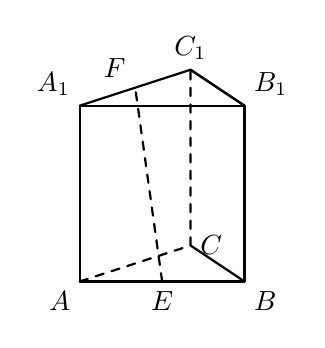
\begin{tikzpicture}[line cap=round,line join=round,x=0.95cm,y=0.95cm]
  \coordinate (A) at (0,0);
  \coordinate (B) at (2.2,0);
  \coordinate (C) at (1.48,0.48);
  \coordinate (Aone) at (0,2.35);
  \coordinate (Bone) at (2.2,2.35);
  \coordinate (Cone) at (1.48,2.83);
  \coordinate (E) at (1.1,0);
  \coordinate (F) at (0.74,2.59);
  \draw[thick] (A)--(B)--(Bone);
  \draw[thick] (A)--(Aone)--(Bone);
  \draw[thick] (Aone)--(Cone)--(Bone);
  \draw[thick] (B)--(C);
  \draw[thick] (Bone)--(Cone);
  \draw[thick,dashed] (A)--(C) (C)--(Cone) (E)--(F);
  \node[below left] at (A) {$A$};
  \node[below right] at (B) {$B$};
  \node[right] at (C) {$C$};
  \node[above left] at (Aone) {$A_1$};
  \node[above right] at (Bone) {$B_1$};
  \node[above] at (Cone) {$C_1$};
  \node[below] at (E) {$E$};
  \node[above left] at (F) {$F$};
\end{tikzpicture}
\end{center}
\nopagebreak[4]
（A）$2$　（B）$\sqrt3$　（C）$\sqrt5$　（D）$\sqrt7$

\Needspace{4\baselineskip}
\textbf{解析}

\Needspace{5\baselineskip}
取底面坐标 $A=(0,0,0), B=(2,0,0), C=(1,\sqrt3,0)$，上底各点的 $z$ 坐标为 $2$。于是 $E=(1,0,0)$，$F$ 为 $A_1(0,0,2)$ 与 $C_1(1,\sqrt3,2)$ 的中点，即 $(1/2,\sqrt3/2,2)$。因此
\nopagebreak[4]
\[
 EF^2=(1/2)^2+(\sqrt3/2)^2+2^2=5,
\]
故 $EF=\sqrt5$，选 C。坐标距离复算符合各棱长为 $2$。

\gkanswer{答案：C，$\sqrt5$。}

\end{answer}
\begin{answer}
\gksolhead{9}{}

\textbf{题目}：

\Needspace{5\baselineskip}
在平面直角坐标系中，不等式组
\nopagebreak[4]
\[
\begin{cases}
x+y-2\geqslant 0,\\
x-y+2\geqslant 0,\\
x\leqslant 2
\end{cases}
\]
表示的平面区域的面积是\mbox{（　　）}

（A）$4\sqrt2$　（B）$4$　（C）$2\sqrt2$　（D）$2$

\Needspace{4\baselineskip}
\textbf{解析}

三条边界围成三角形，顶点为两斜线交点 $(0,2)$，以及它们与 $x=2$ 的交点 $(2,0),(2,4)$。以长为 $4$ 的竖边为底，高为 $2$，面积 $\frac12\cdot4\cdot2=4$，选 B。

\gkanswer{答案：B，$4$。}

\end{answer}
\begin{answer}
\gksolhead{10}{}

\textbf{题目}：

\Needspace{5\baselineskip}
对 $a,b\in\mathbb R$，记
\nopagebreak[4]
\[
\max\{a,b\}=\begin{cases}a,&a\geqslant b,\\b,&a<b,\end{cases}
\]
函数 $f(x)=\max\{|x+1|,|x-2|\}$（$x\in\mathbb R$）的最小值是\mbox{（　　）}

（A）$0$　（B）$\dfrac12$　（C）$\dfrac32$　（D）$3$

\Needspace{4\baselineskip}
\textbf{解析}

两个距离 $|x+1|,|x-2|$ 的最大值在两中心点 $-1,2$ 的中点 $x=1/2$ 处最小；此时两个值均为 $3/2$。任意 $x$ 下两距离之和至少为 $3$，最大者至少为 $3/2$，故最小值为 $3/2$，选 C。

\gkanswer{答案：C，$\dfrac32$。}

\end{answer}
\begin{answer}
\gksolhead{11}{}

\textbf{题目}：

不等式 $\dfrac{x+1}{x-2}>0$ 的解集是\gkblank{}。

\Needspace{4\baselineskip}
\textbf{解析}

临界点为 $-1,2$。分子分母同号时分式为正，得 $x<-1$ 或 $x>2$；$x=2$ 不在定义域，端点 $-1$ 使分子为零，均不取。答案为 $(-\infty,-1)\cup(2,+\infty)$。

\gkanswer{答案：$(-\infty,-1)\cup(2,+\infty)$。}

\end{answer}
\begin{answer}
\gksolhead{12}{}

\textbf{题目}：

函数 $y=2\sin x\cos x-1$，$x\in\mathbb R$ 的值域是\gkblank{}。

\Needspace{4\baselineskip}
\textbf{解析}

$2\sin x\cos x-1=\sin 2x-1$，而 $\sin2x\in[-1,1]$，故值域为 $[-2,0]$。两端分别在 $2x=3\pi/2$ 与 $2x=\pi/2$ 等角处达到。

\gkanswer{答案：$[-2,0]$。}

\end{answer}
\begin{answer}
\gksolhead{13}{}

\textbf{题目}：

双曲线 $\dfrac{x^2}{m}-y^2=1$ 上的点到左焦点的距离与到左准线的距离的比是 $3$，则 $m$ 等于\gkblank{}。

\Needspace{4\baselineskip}
\textbf{解析}

双曲线为 $x^2/a^2-y^2=1$，其中 $a=\sqrt m$、$b=1$、左焦点坐标 $(-c,0)$，$c=\sqrt{m+1}$。对双曲线上任一点，焦点距与对应准线距之比恒为离心率 $e=c/a$。故 $\sqrt{m+1}/\sqrt m=3$，解得 $m+1=9m$，即 $m=1/8$。代回 $c/a=3$。

\gkanswer{答案：$m=\dfrac18$。}

\end{answer}
\begin{answer}
\gksolhead{14}{}

\textbf{题目}：

如图，正四面体 $ABCD$ 的棱长为 $1$，平面 $\alpha$ 过棱 $AB$，且 $CD\parallel\alpha$，则正四面体上的所有点在平面 $\alpha$ 内的射影构成的图形面积是\gkblank{}。
\nopagebreak[4]
\begin{center}% Source: 2006浙江文.pdf, source-relative PDF page 1, Q14.
% The interior label is B' in the scan; the alpha plane and dashed edges are retained.
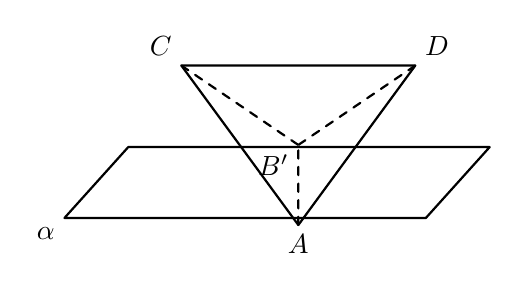
\begin{tikzpicture}[line cap=round,line join=round,x=0.9cm,y=0.9cm]
  \coordinate (C) at (0,2.5);
  \coordinate (D) at (3.3,2.5);
  \coordinate (A) at (1.65,0.25);
  \coordinate (Bp) at (1.65,1.38);
  \coordinate (L) at (-0.75,1.35);
  \coordinate (R) at (4.35,1.35);
  \coordinate (Lb) at (-1.65,0.35);
  \coordinate (Rb) at (3.45,0.35);
  \draw[thick] (L)--(R)--(Rb)--(Lb)--cycle;
  \draw[thick] (C)--(D) (C)--(A) (D)--(A);
  \draw[thick,dashed] (C)--(Bp) (D)--(Bp) (A)--(Bp);
  \node[above left] at (C) {$C$};
  \node[above right] at (D) {$D$};
  \node[below] at (A) {$A$};
  \node[below left] at (Bp) {$B'$};
  \node[below left] at (Lb) {$\alpha$};
\end{tikzpicture}
\end{center}
\nopagebreak[4]
\Needspace{4\baselineskip}
\textbf{解析}

设 $A=(0,0,0),B=(1,0,0),C=(1/2,\sqrt3/2,0),D=(1/2,\sqrt3/6,\sqrt{2/3})$。$CD$ 是单位方向向量 $u=(0,-\sqrt3/3,\sqrt{2/3})$，平面 $\alpha$ 由 $AB$ 方向与 $u$ 方向张成。正交投影到该平面后，$A,B$ 不动；以 $u$ 为平面内第二坐标轴，$C,D$ 的投影坐标分别为 $(1/2,-1/2),(1/2,1/2)$。四投影构成顶点 $(0,0),(1,0),(1/2,1/2),(1/2,-1/2)$ 的菱形，面积为 $1/2$。按鞋带公式复算面积也是 $1/2$。

\gkanswer{答案：$\dfrac12$。}

\end{answer}
\begin{answer}
\gksolhead{15}{}

\textbf{题目}：

若 $S_n$ 是公差不为 $0$ 的等差数列 $\{a_n\}$ 的前 $n$ 项和，且 $S_1,S_2,S_4$ 成等比数列。

（1） 求数列 $S_1,S_2,S_4$ 的公比；

（2） 若 $S_2=4$，求 $\{a_n\}$ 的通项公式。

\Needspace{4\baselineskip}
\textbf{解析}

\gksubpart{（1）}

\Needspace{5\baselineskip}
设 $a_1=a,d\ne0$。则 $S_1=a,S_2=2a+d,S_4=4a+6d$。等比条件给出
\nopagebreak[4]
\[
 (2a+d)^2=a(4a+6d),
\]
化简为 $d^2=2ad$。因 $d\ne0$，$d=2a$，故 $S_2/S_1=4$。三个和分别为 $a,4a,16a$，复算公比均为 $4$。

\gksubpart{（2）}

由 $S_2=4$ 且 $S_2=4a$，得 $a=1$、$d=2$。于是 $a_n=1+2(n-1)=2n-1$，回代前两项和 $S_2=1+3=4$。

\gkanswer{答案（1）：$4$。}

\gkanswer{答案（2）：$a_n=2n-1$。}

\end{answer}
\begin{answer}
\gksolhead{16}{}

\textbf{题目}：

如图，函数 $y=2\sin(\pi x+\varphi)$，$x\in\mathbb R$（其中 $0\leqslant\varphi\leqslant\dfrac\pi2$）的图象与 $y$ 轴交于点 $(0,1)$。

（1） 求 $\varphi$ 的值；

（2） 设 $P$ 是图象上的最高点，$M,N$ 是图象与 $x$ 轴的交点，求 $\overrightarrow{PM}$ 与 $\overrightarrow{PN}$ 的夹角。
\nopagebreak[4]
\begin{center}% Source: 2006浙江文.pdf, source-relative PDF page 1, Q16.
% Preserve the adjacent zeros M and N around the labelled maximum P and y=1 level.
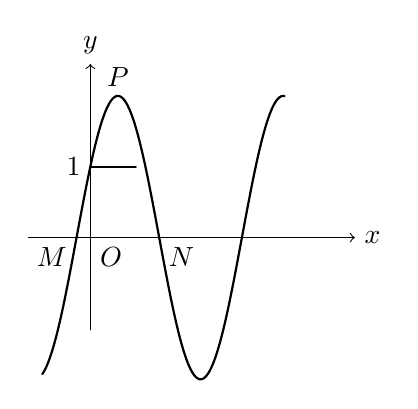
\begin{tikzpicture}[line cap=round,line join=round,x=1.05cm,y=0.9cm]
  \draw[->] (-0.75,0)--(3.2,0) node[right] {$x$};
  \draw[->] (0,-1.3)--(0,2.45) node[above] {$y$};
  \draw[thick] plot[domain=-0.58:2.35,samples=140] (\x,{2*sin(180*\x+30)});
  \draw[thick] (0,1)--(0.55,1);
  \node[left] at (0,1) {$1$};
  \node[above] at (1/3,2) {$P$};
  \node[below left] at (-1/6,0) {$M$};
  \node[below right] at (5/6,0) {$N$};
  \node[below right] at (0,0) {$O$};
\end{tikzpicture}
\end{center}
\nopagebreak[4]
\Needspace{4\baselineskip}
\textbf{解析}

\gksubpart{（1）}

令 $x=0$，得 $2\sin\varphi=1$。由 $0\le\varphi\le\pi/2$，$\varphi=\pi/6$。

\gksubpart{（2）}

最高点横坐标满足 $\pi x+\pi/6=\pi/2+2k\pi$，故可取 $P=(1/3,2)$。零点满足 $x=j-1/6$，$j\in\mathbb Z$；原页图明确标出 $P$ 左右相邻的两个零点 $M,N$，并画出 $PM,PN$，故可取 $M=(-1/6,0),N=(5/6,0)$。于是 $\overrightarrow{PM}=(-1/2,-2)$、$\overrightarrow{PN}=(1/2,-2)$，点积为 $15/4$，模长平方均为 $17/4$，故夹角余弦为 $15/17$，夹角为 $\arccos(15/17)$。点积与模长回算一致。

\gkanswer{答案（1）：$\varphi=\dfrac\pi6$。}

\gkanswer{答案（2）：$\arccos\dfrac{15}{17}$。}

\end{answer}
\begin{answer}
\gksolhead{17}{}

\textbf{题目}：

如图，在四棱锥 $P-ABCD$ 中，底面为直角梯形，$AD\parallel BC$，$\angle BAD=90^\circ$，$PA\perp$ 底面 $ABCD$，且 $PA=AD=AB=2BC$，$M,N$ 分别为 $PC,PB$ 的中点。

（1） 求证：$PB\perp DM$；

（2） 求 $BD$ 与平面 $ADMN$ 所成的角。
\nopagebreak[4]
\begin{center}% Source: 2006浙江文.pdf, source-relative PDF page 1, Q17.
% Vertex labels and solid/dashed edge relationships follow the printed projection.
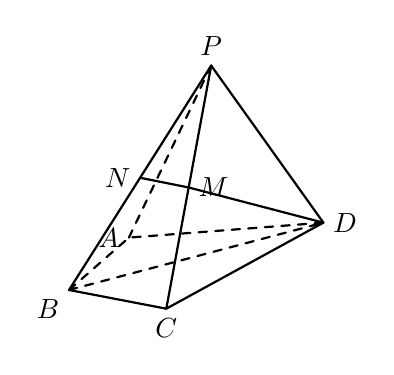
\begin{tikzpicture}[line cap=round,line join=round,x=0.95cm,y=0.95cm]
  \coordinate (P) at (1.65,3.15);
  \coordinate (A) at (0.55,0.85);
  \coordinate (B) at (-0.25,0.15);
  \coordinate (C) at (1.05,-0.1);
  \coordinate (D) at (3.15,1.05);
  \coordinate (N) at (0.7,1.65);
  \coordinate (M) at (1.35,1.52);
  \draw[thick] (P)--(B)--(C)--(D)--cycle;
  \draw[thick] (P)--(C) (N)--(M)--(D);
  \draw[thick,dashed] (P)--(A) (B)--(A)--(D) (B)--(D);
  \node[above] at (P) {$P$};
  \node[left] at (A) {$A$};
  \node[below left] at (B) {$B$};
  \node[below] at (C) {$C$};
  \node[right] at (D) {$D$};
  \node[left] at (N) {$N$};
  \node[right] at (M) {$M$};
\end{tikzpicture}
\end{center}
\nopagebreak[4]
\Needspace{4\baselineskip}
\textbf{解析}

\gksubpart{（1）}

令 $A=(0,0,0),D=(2,0,0),B=(0,2,0),C=(1,2,0),P=(0,0,2)$，满足直角梯形尺寸关系。$M=(P+C)/2=(1/2,1,1)$。取 $\overrightarrow{PB}=(0,2,-2)$、$\overrightarrow{DM}=(-3/2,1,1)$，内积为 $0+2-2=0$，故 $PB\perp DM$。且 $|AB|=|AD|=|PA|=2, |BC|=1$，与题设相符。

\gksubpart{（2）}

\Needspace{5\baselineskip}
中点 $N=(P+B)/2=(0,1,1)$。平面 $ADMN$ 过 $x$ 轴及点 $N$，方程为 $y=z$，法向量可取 $(0,1,-1)$。$\overrightarrow{BD}=(2,-2,0)$，于是线面角 $\theta$ 满足
\nopagebreak[4]
\[
\sin\theta=\frac{|\overrightarrow{BD}\cdot(0,1,-1)|}{|BD|\sqrt2}=\frac{2}{2\sqrt2\cdot\sqrt2}=\frac12,
\]
故 $\theta=30^\circ$。代回平面方程，$A,D,M,N$ 均满足 $y=z$。

\gkanswer{答案（1）：见解析版}

\gkanswer{答案（2）：$30^\circ$。}

\end{answer}
\begin{answer}
\gksolhead{18}{}

\textbf{题目}：

甲、乙两袋装有大小相同的红球和白球，甲袋装有 $2$ 个红球、$2$ 个白球，乙袋装有 $2$ 个红球、$n$ 个白球。现从甲、乙两袋中各任取 $2$ 个球。

（1） 若 $n=3$，求取到的 $4$ 个球全是红球的概率；

（2） 若取到的 $4$ 个球中至少有 $2$ 个红球的概率为 $\dfrac34$，求 $n$。

\Needspace{4\baselineskip}
\textbf{解析}

\gksubpart{（1）}

甲袋两球全红的概率为 $1/\binom42=1/6$；$n=3$ 时乙袋两球全红概率亦为 $1/\binom52=1/10$。两袋独立，所求为 $1/60$。

\gksubpart{（2）}

\Needspace{5\baselineskip}
甲袋抽到 $0,1,2$ 个红球的概率依次为 $1/6,2/3,1/6$。设乙袋两球中零红球和恰一红球的概率分别为
\nopagebreak[4]
\[
q=\frac{\binom n2}{\binom{n+2}2}=\frac{n(n-1)}{(n+1)(n+2)},\qquad
r=\frac{2n}{\binom{n+2}2}=\frac{4n}{(n+1)(n+2)}.
\]
\Needspace{5\baselineskip}
总红球少于两球的情况是：甲抽 0 红且乙抽 0 红、甲抽 1 红且乙抽 0 红、甲抽 0 红且乙恰抽 1 红。因此互补概率为 $\frac16q+\frac23q+\frac16r=\frac56q+\frac16r$。令其为 $1/4$，代入得
\nopagebreak[4]
\[
\frac{5n(n-1)+4n}{6(n+1)(n+2)}=\frac14,
\]
化简为 $7n^2-11n-6=0$，正根为 $n=2$。复算：$n=2$ 时 $q=1/6,r=2/3$，少于两红概率为 $5/36+4/36=1/4$，故至少两红概率为 $3/4$。

\gkanswer{答案（1）：$\dfrac1{60}$。}

\gkanswer{答案（2）：$n=2$。}

\end{answer}
\begin{answer}
\gksolhead{19}{}

\textbf{题目}：

如图，椭圆 $\dfrac{x^2}{a^2}+\dfrac{y^2}{b^2}=1$（$a>b>0$）与过点 $A(2,0),B(0,1)$ 的直线有且只有一个公共点 $T$，且椭圆的离心率 $e=\dfrac{\sqrt3}{2}$。

（1） 求椭圆方程；

（2） 设 $F_1,F_2$ 分别为椭圆的左、右焦点，求证：$|AT|^2=\dfrac12|AF_1|\cdot|AF_2|$。
\nopagebreak[4]
\begin{center}% Source: 2006浙江文.pdf, source-relative PDF page 2, Q19.
% Preserve the labelled ellipse, axes, foci, A/B and the straight line AB through T.
\begin{tikzpicture}[line cap=round,line join=round,x=0.85cm,y=0.85cm]
  \draw[->] (-3.8,0)--(4.2,0) node[right] {$x$};
  \draw[->] (0,-2.7)--(0,2.7) node[above] {$y$};
  \draw[thick] (0,0) ellipse (2.45 and 1.225);
  \coordinate (A) at (3.4,0);
  \coordinate (B) at (0,1.7);
  \coordinate (T) at (1.7,0.85);
  \coordinate (Fone) at (-2.121,0);
  \coordinate (Ftwo) at (2.121,0);
  \draw[thick] (B)--(A);
  \fill (Fone) circle (1.4pt);
  \fill (Ftwo) circle (1.4pt);
  \node[above left] at (B) {$B$};
  \node[above right] at (T) {$T$};
  \node[below] at (A) {$A$};
  \node[below left] at (Fone) {$F_1$};
  \node[below right] at (Ftwo) {$F_2$};
  \node[below left] at (0,0) {$O$};
\end{tikzpicture}
\end{center}
\nopagebreak[4]
\Needspace{4\baselineskip}
\textbf{解析}

\gksubpart{（1）}

离心率给出 $c^2/a^2=3/4$，所以 $b^2=a^2/4$。直线 $AB$ 为 $x/2+y=1$。椭圆在法向量 $(1/2,1)$ 方向的支撑函数值为 $\sqrt{a^2/4+b^2}$，该直线与椭圆相切当且仅当 $a^2/4+b^2=1$。代入 $b^2=a^2/4$ 得 $a^2/2=1$，故 $a^2=2,b^2=1/2$，椭圆方程为 $x^2/2+2y^2=1$。切点坐标为 $(a^2/2,b^2)=(1,1/2)$，代入椭圆左边为 $1/2+1/2=1$。

\gksubpart{（2）}

由切点条件 $T=(1,1/2)$，$|AT|^2=(1-2)^2+(1/2)^2=5/4$。$c=ae=\sqrt6/2$，焦点为 $(\pm\sqrt6/2,0)$。因此 $|AF_1|=2+\sqrt6/2$、$|AF_2|=2-\sqrt6/2$，乘积为 $4-c^2=4-3/2=5/2$，其一半为 $5/4=|AT|^2$。直接平方复算命题。

\gkanswer{答案（1）：$\dfrac{x^2}{2}+2y^2=1$。}

\gkanswer{答案（2）：见解析版}

\end{answer}
\begin{answer}
\gksolhead{20}{}

\textbf{题目}：

设 $f(x)=3ax^2+2bx+c$，若 $a+b+c=0$，$f(0)f(1)>0$，求证：

（1） 方程 $f(x)=0$ 有实根；

（2） $-2<\dfrac ba<-1$；

（3） 设 $x_1,x_2$ 是方程 $f(x)=0$ 的两个实根，则 $\dfrac{\sqrt3}{3}\leqslant|x_1-x_2|<\dfrac23$。

\Needspace{4\baselineskip}
\textbf{解析}

\gksubpart{（1）}

\Needspace{5\baselineskip}
由 $a+b+c=0$ 得 $c=-a-b$，而 $f(0)f(1)=c(2a+b)>0$，故 $a\ne0$。令 $t=b/a$，则
\nopagebreak[4]
\[
 c(2a+b)=-a^2(1+t)(2+t)>0,
\]
从而 $(1+t)(2+t)<0$，即 $-2<t<-1$。令 $g(t)=t^2+3t+3=(t+3/2)^2+3/4>0$，则方程判别式为 $4g(t)>0$，故方程有两个实根。

\gksubpart{（2）}

因 $a\ne0$，令 $t=b/a$。由 $f(0)f(1)=-a^2(1+t)(2+t)>0$ 得 $(1+t)(2+t)<0$，所以 $-2<t<-1$。

\gksubpart{（3）}

\Needspace{5\baselineskip}
将 $c=-a-b$ 代入 $f(x)=0$ 并除以 $a$，得 $3x^2+2tx-(1+t)=0$，其判别式为 $4g(t)$，其中 $g(t)=t^2+3t+3=(t+3/2)^2+3/4$。在 $-2<t<-1$ 上有 $3/4\le g(t)<1$。两根差的绝对值为
\nopagebreak[4]
\[
 |x_1-x_2|=\frac{\sqrt{4g(t)}}{3}=\frac23\sqrt{g(t)}.
\]
于是 $\sqrt3/3\le |x_1-x_2|<2/3$。下界在 $t=-3/2$ 达到；上界只在区间端点可逼近而不能达到。重算判别式与韦达根差公式一致。

\gkanswer{答案（1）：方程有两个实根。}

\gkanswer{答案（2）：$-2<\dfrac ba<-1$。}

\gkanswer{答案（3）：$\dfrac{\sqrt3}{3}\leqslant|x_1-x_2|<\dfrac23$。}

\end{answer}